
The FSM dictates how control is coordinated amongst the different controllers and 
is responsible for sending the appropriate actuator value to the BASE node. 
Figure~\ref{fig:fsm_radl} shows part of the RADL architecture containing the FSM node 
and the nodes connected to it.

\begin{figure}[ht]
  \centering
  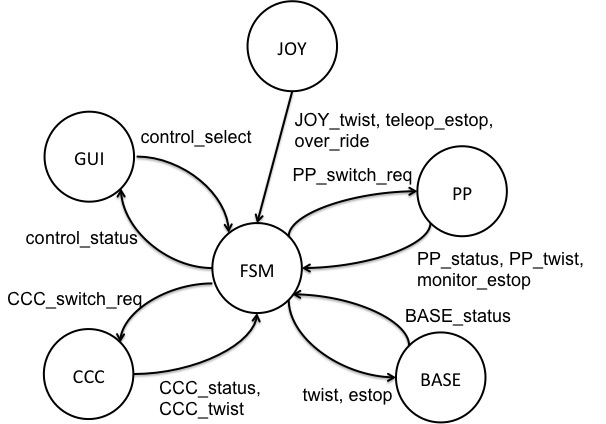
\includegraphics[width=0.7\textwidth]{figures/fsm_radl.jpg}
  \caption{The FSM arbitrates the switch amongst the three controllers -- Constant Cruise Controller (CCC), Path Planner (PP) and Joystick (JOY). Based on the arbitration result, it then sends the appropriate twist (linear and angular velocity) message to the BASE node.}
  \label{fig:fsm_radl}
\end{figure}

There are currently 5 RADL nodes connected to the FSM. 
Among these, CCC, PP and JOY are the controllers, each producing its own twist message. 
CCC and PP are autonomous controller and JOY corresponds to manual input generated by a user operating the joystick. 
During normal operation, the user can select a controller to control the vehicle by setting the \texttt{control\_select} signal from the GUI.
The FSM may also receive a \texttt{ESTOP} message in a scenario where emergency stop is required.  
Currently, there are two \texttt{ESTOP} messages -- one produced by the monitor (\texttt{monitor\_estop}) 
and sent to the FSM through the PP node, and the other from the joystick (\texttt{teleop\_estop}). 
Hence, the FSM maintains 4 control modes -- \texttt{CCC}, \texttt{PP}, \texttt{JOY} and \texttt{ESTOP}. 
The FSM also publishes its current control mode through the \texttt{control\_status} message to the GUI. 
Depending on which control mode it is in, the FSM forwards the corresponding twist message to the BASE. 
For instance, if the FSM is in \texttt{CCC} mode, then it sets \texttt{twist} to \texttt{CCC\_twist}. 
%In addition, if it receives a \texttt{ESTOP} message in this mode, then it will also forward it to the BASE.
The \texttt{over\_ride} message behaves in a similar way as a control select on the joystick -- when it is set, 
the FSM should switch to the \texttt{JOY} mode as soon as possible. 

\noindent
{\bf Control priority.}
Control priority determines the conditions under which the FSM should switch to a particular mode. 
Manual control always supersedes other control modes. Note that this also means the user can use the joystick to move the vehicle
when it is in the \texttt{ESTOP} mode. 
\texttt{ESTOP} has a higher priority than any of the two auto modes but a lower priority than manual control. 
This means the \texttt{ESTOP} mode can be entered when the FSM is currently in one of the two auto modes (\texttt{CCC} or \texttt{PP}) and 
receives a \texttt{teleop\_estop} message set to true (currently \texttt{monitor\_estop} only takes effect when the FSM is in the \texttt{PP} mode).
In addition, the FSM can enter the \texttt{ESTOP} mode if it receives a \texttt{teleop\_estop} message in the \texttt{JOY} mode
(given that the joystick is not selected simultaneously either through the \texttt{control\_select} signal or through setting the 
\texttt{over\_ride} message). 
The two auto modes have equal priority. This means if the FSM is in \texttt{CCC} mode, then it cannot directly jump to the \texttt{PP} mode 
and vice versa. Figure~\ref{fig:fsm_mode} shows the possible transitions among the 4 modes. 

\begin{figure}[ht]
  \centering
  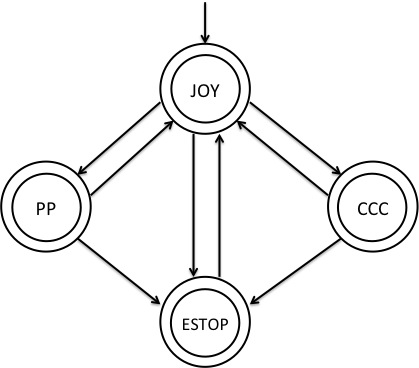
\includegraphics[width=0.5\textwidth]{figures/fsm_mode.jpg}
  \caption{Possible FSM mode transitions. Initially, the FSM is in JOY mode (manual control).}
  \label{fig:fsm_mode}
\end{figure}

\noindent
{\bf Control handshake.}
When the user selects one of the two auto modes (from the \texttt{JOY} mode), 
the FSM will first perform a handshake with the corresponding controller before control can be established for that controller. 
For instance, if the user tries to set the vehicle to constant speed control by setting \texttt{control\_select}, 
the FSM will first send a request (setting the \texttt{CCC\_switch\_req} message to appropriate value) to CCC. 
It then waits for an engage signal (the \texttt{CCC\_status} will be set to \texttt{ENGAGE\_GUARANTEE} or 
\texttt{ENGAGE\_NO\_GUARANTEE}) from the CCC controller for a small number of periods (e.g., $3$). 
If it receives the engage signal within the waiting time, the FSM will transition to the \texttt{CCC} control mode and set the 
actuator output to the BASE (\texttt{twist}) to the value computed by the CCC controller (\texttt{CCC\_twist}) in the same period. 
Otherwise, it stays in the \texttt{JOY} control mode. 
